\begin{frame}{Soluciones aproximadas de la ecuación de Navier Stokes}
\justifying

\begin{figure}[H]
\centering
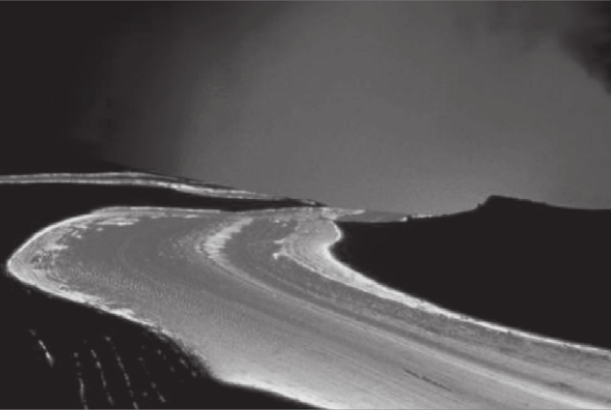
\includegraphics[scale=0.2]{Section_Files/S3-imagenes-Jhon/0001.png}
\caption{El flujo de lava de un volcán es un ejemplo de flujo trepador: la viscosidad de la roca fundida es tan grande que el número de Reynolds es pequeño aún cuando las escalas de longitud sean grandes.}
\end{figure}

{\tiny Mecánica de fluidos por Yunus A. Cengel, John M. Cimbala, pág. 491}
\end{frame}

%***************************
\begin{frame}{01. Introducción 01/03}
\justifying
La mayoría de los problemas prácticos de la mecánica de fluidos no puede resolverse de manera analítica y demanda ya sea 1) mayores aproximaciones o 2) ayuda de computadora. Consideraremos a los flujos en estudio como incompresibles del tipo de fluido newtonianos.

%La ecuación de Navier-Stokes no es exacta por si misma, sino que se trata de un modelo de flujo de fluidos que incluye varias aproximaciones inherentes (fluido newtoniano, propiedades termodinámicas y de transporte constante, etc.). No obstante, es un excelente modelo y fundamento de la mecánica de fluidos moderna, Ahora distinguiremos entre soluciones "exactas" y soluciones aproximadas. El termino exacto se utiliza cuando la solución comienza con la ecuación de Navier-Stokes completa. Existen casos en los que algunos terminos se eliminan debido a la geometría especificada u otras hipótesis de simplificación en el problema.

Una solución aproximada se define como aquella donde la ecuación de Navier-Stokes se simplifica en alguna región del flujo antes de inclusive comenzar la solución. En otras palabras se comienzan a eliminar terminos dependiendo de la clase de problema, el cual puede diferir una región del flujo a otra.


Los fluidos estáticos pueden considerarse como una solución aproximada de Navier-Stokes. La aproximación es que los términos inercial y viscoso en la ecuación de Navier-Stokes son despreciablemente pequeños en comparación con los términos de presión y gravedad.
{\tiny Mecánica de fluidos por Yunus A. Cengel, John M. Cimbala, pág. 492}
\end{frame}

\begin{frame}{01. Introducción 02/03}
\justifying
\begin{figure}[H]
\centering
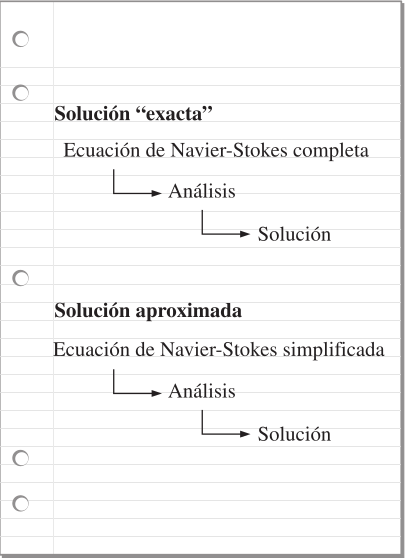
\includegraphics[scale=0.2]{Section_Files/S3-imagenes-Jhon/0002.png}
\caption{Las soluciones "exactas" comienzan con la ecuación de Navier-Stokes completa, mientras que las soluiciones aproximadas comienzan con una forma simplificada de la ecuación de Navier-Stokes justo desde el principio.}
\end{figure}

{\tiny Mecánica de fluidos por Yunus A. Cengel, John M. Cimbala, pág. 492}
\end{frame}

\begin{frame}{01. Introducción 03/03}
\justifying
\begin{figure}[H]
\centering
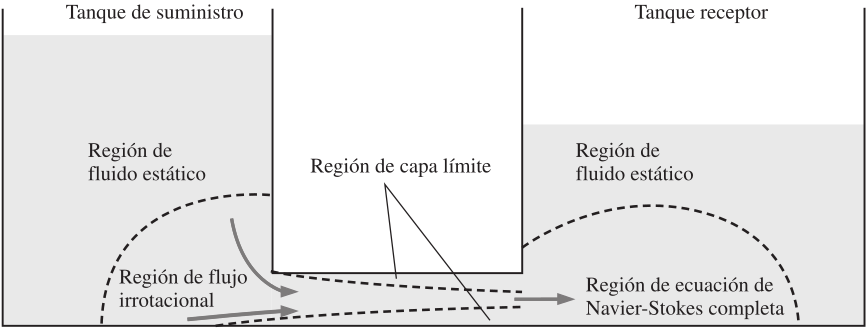
\includegraphics[scale=0.2]{Section_Files/S3-imagenes-Jhon/0003.png}
\caption{Una aproximación partícular de la ecuación de Navier-Stokes es adecuada sólo en ciertas regiones del campo de flujo; otras aproximaciones pueden no ser adecuadas en otras regiones del campo de flujo.}
\end{figure}

{\tiny Mecánica de fluidos por Yunus A. Cengel, John M. Cimbala, pág. 493}
\end{frame}


%***************************

\begin{frame}{02. Ecuaciones adimensionalizadas de movimiento 01/04}
\justifying
Se desea eliminar las dimensiones de las ecuaciones de movimiento, de modo que puedan compararse de manera adecuada las órdenes de magnitud de los diversos términos de las ecuaciones, para ello comenzamos con la ecuación de continuidad de flujo incompresible:
\begin{figure}[H]
\centering
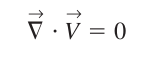
\includegraphics[scale=0.2]{Section_Files/S3-imagenes-Jhon/0004.png}
\end{figure}
y la forma vectorial de la ecuación de Navier-Stokes, valida para flujo incompresible de un fluido newtoniano con propiedades constantes:
\begin{figure}[H]
\centering
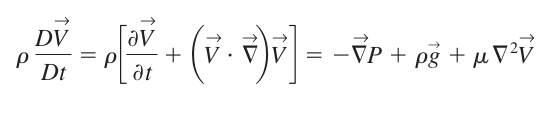
\includegraphics[scale=0.2]{Section_Files/S3-imagenes-Jhon/0005.png}
\end{figure}
{\tiny Mecánica de fluidos por Yunus A. Cengel, John M. Cimbala, pág. 493}
\end{frame}

\begin{frame}{02. Ecuaciones adimensionalizadas de movimiento 02/04}
\justifying
Mostramos algunos parámetros de escalamiento o repetitivas característicos que se usan para eliminar las dimensiones de las ecuaciones de movimiento.
\begin{figure}[H]
\centering
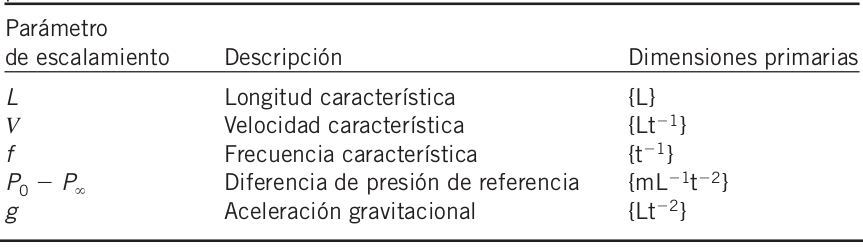
\includegraphics[scale=0.3]{Section_Files/S3-imagenes-Jhon/0006.png}
\end{figure}
{\tiny Mecánica de fluidos por Yunus A. Cengel, John M. Cimbala, pág. 494}
\end{frame}

\begin{frame}{02. Ecuaciones adimensionalizadas de movimiento 03/04}
\justifying
Luego se definen algunas variables adimensionales y un operador adimensional con base en los parámetros de escalamiento de la tabla mostrada en el slider anterior.
\begin{figure}[H]
\centering
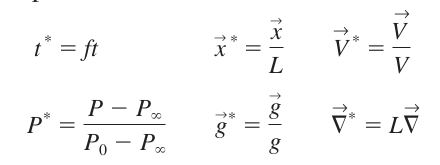
\includegraphics[scale=0.3]{Section_Files/S3-imagenes-Jhon/0007.png}
\end{figure}
{\tiny Mecánica de fluidos por Yunus A. Cengel, John M. Cimbala, pág. 494}
\end{frame}

\begin{frame}{02. Ecuaciones adimensionalizadas de movimiento 04/04}
\justifying
Luego de haber multiplicado los terminos de la ecuación de Navier-Stokes por sus respectivos factores se obtiene.
\begin{figure}[H]
\centering
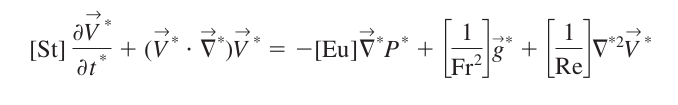
\includegraphics[scale=0.3]{Section_Files/S3-imagenes-Jhon/0015.png}
\end{figure}
{\tiny Mecánica de fluidos por Yunus A. Cengel, John M. Cimbala, pág. 495}
\end{frame}


%***************************

\begin{frame}{03. Aproximación de flujo de Stokes}
\justifying
\begin{figure}[H]
\centering
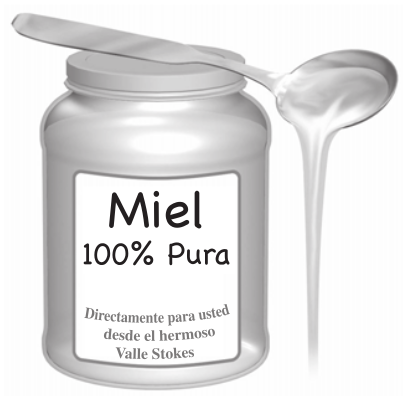
\includegraphics[scale=0.35]{Section_Files/S3-imagenes-Jhon/0022.png}
\caption{El lento flujo de un líquido muy viscoso, en este caso la miel, se clasifica como flujo de Stokes.}
\end{figure}
%\\
{\tiny Mecánica de fluidos por Yunus A. Cengel, John M. Cimbala, pág. 496}
\end{frame}

%***************************

\begin{frame}{Fuerza de arrastre sobre una esfera en flujo de Stokes}
\justifying
\begin{figure}[H]
\centering
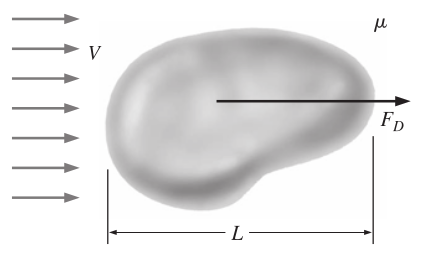
\includegraphics[scale=0.35]{Section_Files/S3-imagenes-Jhon/0031.png}
\caption{Para flujo de Stokes sobre un objeto tridimensional la fuerza de arrastre sobre el objeto no depende de la densidad, sino sólo de la velocidad V, alguna longitud característica del objeto $ L $ y la viscosidad del fluido $ \mu $.}
\end{figure}
{\tiny Mecánica de fluidos por Yunus A. Cengel, John M. Cimbala, pág. 499}
\end{frame}

%***************************

\begin{frame}{04. Aproximación para regiones invíscidas de flujo}
\justifying
\begin{figure}[H]
\centering
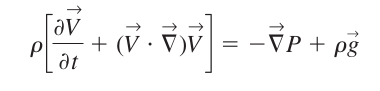
\includegraphics[scale=0.35]{Section_Files/S3-imagenes-Jhon/0035.png}
\caption{Ecuación de Euler.}
\end{figure}
{\tiny Mecánica de fluidos por Yunus A. Cengel, John M. Cimbala, pág. 501}
\end{frame}

%***************************

\begin{frame}{Derivación de la ecuación de Bernoulli en regiones inviscidas de flujo}
\justifying
\begin{figure}[H]
\centering
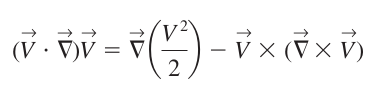
\includegraphics[scale=0.35]{Section_Files/S3-imagenes-Jhon/0037.png}
\caption{Ecuación de Euler.}
\end{figure}
{\tiny Mecánica de fluidos por Yunus A. Cengel, John M. Cimbala, pág. 502}
\end{frame}

%***************************

\begin{frame}{05. La aproximación de flujo irrotacional}
\justifying
\begin{figure}[H]
\centering
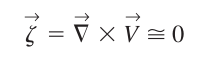
\includegraphics[scale=0.35]{Section_Files/S3-imagenes-Jhon/0048.png}
\caption{Aproximación irrotacional.}
\end{figure}
{\tiny Mecánica de fluidos por Yunus A. Cengel, John M. Cimbala, pág. 505}
\end{frame}

%***************************

\begin{frame}{Ecuación de continuidad}
\justifying
\begin{figure}[H]
\centering
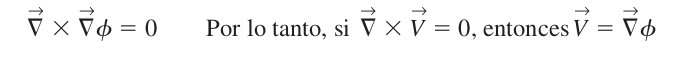
\includegraphics[scale=0.35]{Section_Files/S3-imagenes-Jhon/0049.png}
\caption{Identidad vectorial.}
\end{figure}
{\tiny Mecánica de fluidos por Yunus A. Cengel, John M. Cimbala, pág. 505}
\end{frame}

%***************************

\begin{frame}{Ecuación de cantidad de movimiento}
\justifying
\begin{figure}[H]
\centering
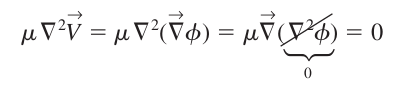
\includegraphics[scale=0.35]{Section_Files/S3-imagenes-Jhon/0060.png}
%\caption{.}
\end{figure}
{\tiny Mecánica de fluidos por Yunus A. Cengel, John M. Cimbala, pág. 507}
\end{frame}

%***************************

\begin{frame}{Deducción de la ecuación de Bernoulli en regiones irrotacionales de flujo}
\justifying
\begin{figure}[H]
\centering
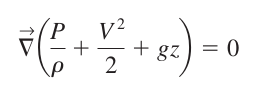
\includegraphics[scale=0.35]{Section_Files/S3-imagenes-Jhon/0062.png}
%\caption{}
\end{figure}
{\tiny Mecánica de fluidos por Yunus A. Cengel, John M. Cimbala, pág. 507}
\end{frame}

%***************************

\begin{frame}{Regiones irrotacionales bidimensionales de flujo}
\justifying
En regiones irrotacionales de flujo...
\\
{\tiny Mecánica de fluidos por Yunus A. Cengel, John M. Cimbala, pág. 510}
\end{frame}

%***************************

\begin{frame}{Regiones de flujo planar irrotacional}
\justifying
\begin{figure}[H]
\centering
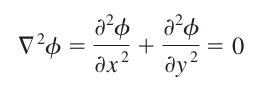
\includegraphics[scale=0.35]{Section_Files/S3-imagenes-Jhon/0072.png}
%\caption{}
\end{figure}
{\tiny Mecánica de fluidos por Yunus A. Cengel, John M. Cimbala, pág. 511}
\end{frame}

%***************************

\begin{frame}{Regiones irrotacionales de flujo aximétrico}
\justifying
\begin{figure}[H]
\centering
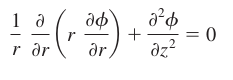
\includegraphics[scale=0.35]{Section_Files/S3-imagenes-Jhon/0081.png}
%\caption{}
\end{figure}
{\tiny Mecánica de fluidos por Yunus A. Cengel, John M. Cimbala, pág. 512}
\end{frame}

%***************************

\begin{frame}{Resumen de regiones irrotacionales de flujo bidimensional}
\justifying
Componentes de velocidad para regiones irrotacionales de flujo bidimensional y estacionario de fluido incompresible en términos de función potencial de velocidad y función de corriente en varios sistemas coordenados.
\begin{figure}[H]
\centering
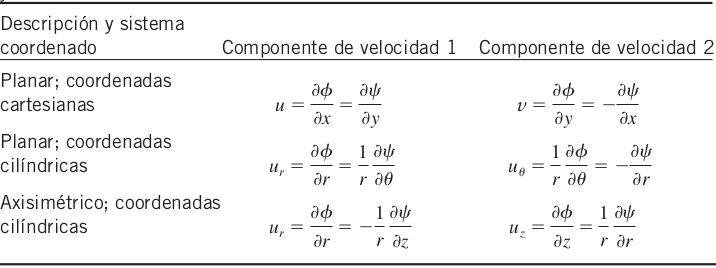
\includegraphics[scale=0.35]{Section_Files/S3-imagenes-Jhon/0088.png}
%\caption{}
\end{figure}
{\tiny Mecánica de fluidos por Yunus A. Cengel, John M. Cimbala, pág. 513}
\end{frame}

%***************************

\begin{frame}{Superposición de flujo en regiones irrotacionales}
\justifying
\begin{figure}[H]
\centering
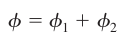
\includegraphics[scale=0.35]{Section_Files/S3-imagenes-Jhon/0091.png}
\caption{Superposición de dos campos de flujo irrotacional}
\end{figure}
{\tiny Mecánica de fluidos por Yunus A. Cengel, John M. Cimbala, pág. 451}
\end{frame}

%***************************

\begin{frame}{Flujo planares irrotacionales elementales}
\justifying
La superposición permite sumar dos o más soluciones simples de flujo irrotacional, para crear un campo de flujo más complejo (y con la esperanza de ser más significativo físicamente). Por lo tanto, es útil establecer una colección de flujos irrotacionales que sirvan como bloques de la construcción elemental con los que se pueda construir una diversidad de flujos más prácticos...
\\
{\tiny Mecánica de fluidos por Yunus A. Cengel, John M. Cimbala, pág. 514}
\end{frame}


%***************************

\begin{frame}{Flujo irrotacional formados por superposición}
\justifying
Ahora se tiene un conjunto de flujos irrotacionales de bloques de construcción, y se está listo para construir algunos campos de flujo irrotacionales más interesantes mediante la técnica de superposición.
{\tiny Mecánica de fluidos por Yunus A. Cengel, John M. Cimbala, pág. 521}
\end{frame}

%***************************

\begin{frame}{Superposición de un sumidero lineal y un vórtice lineal}
\justifying
\begin{figure}[H]
\centering
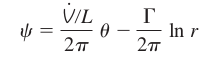
\includegraphics[scale=0.35]{Section_Files/S3-imagenes-Jhon/0132.png}
\caption{Superposición.}
\end{figure}
{\tiny Mecánica de fluidos por Yunus A. Cengel, John M. Cimbala, pág. 521}
\end{frame}

%***************************

\begin{frame}{Superposición de un flujo uniforme y un doblete: flujo sobre un cilindro circular}
\justifying
\begin{figure}[H]
\centering
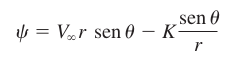
\includegraphics[scale=0.35]{Section_Files/S3-imagenes-Jhon/0137.png}
\caption{Superposición.}
\end{figure}
{\tiny Mecánica de fluidos por Yunus A. Cengel, John M. Cimbala, pág. 522}
\end{frame}

%***************************

\begin{frame}{06. La aproximación de capa límite}
\justifying

\begin{figure}
\centering
\subfloat[Entre la ecuación de Euler (que permite el deslizamiento en las paredes) y la ecuación de Navier-Stokes (que apoya la condición de no deslizamiento) existe un gran vacío.]{
%\label{f:imagen01}
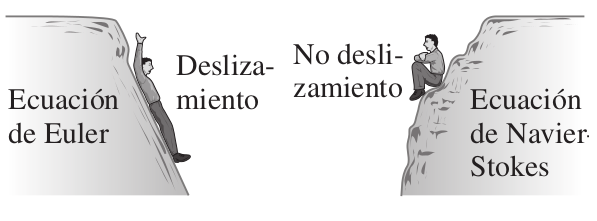
\includegraphics[scale=0.20]{Section_Files/S3-imagenes-Jhon/0163.png}}
\subfloat[La aproximación de capa límite tiende un puente entre ese vacío.]{
%\label{f:imagen02}
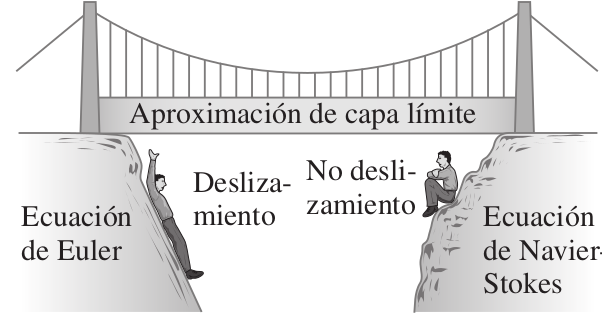
\includegraphics[scale=0.20]{Section_Files/S3-imagenes-Jhon/0164.png}}
%\caption{Imagenes}
%\label{f:imagenes01}

\end{figure}

{\tiny Mecánica de fluidos por Yunus A. Cengel, John M. Cimbala, pág. 451}
\end{frame}

%***************************

\begin{frame}{Ecuaciones de la capa límite}
\justifying
\begin{figure}[H]
\centering
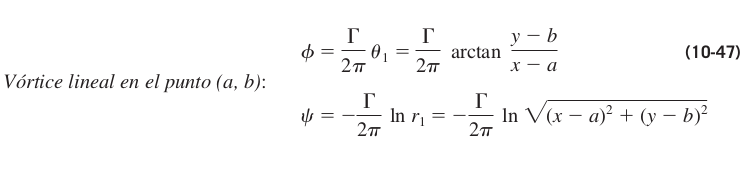
\includegraphics[scale=0.25]{Section_Files/S3-imagenes-Jhon/0123.png}
\caption{Sistema coordenado para capa límite de flujo sobre un cuerpo; $ x $ sigue la superficie y, por lo general, se establece en cero el punto de estancamiento frontal del cuerpo, y $ y $ localmente es normal a la superficie en todas partes.}
\end{figure}
{\tiny Mecánica de fluidos por Yunus A. Cengel, John M. Cimbala, pág. 535}
\end{frame}

%***************************

\begin{frame}{El procedimiento de capa límite}
\justifying
\begin{figure}[H]
\centering
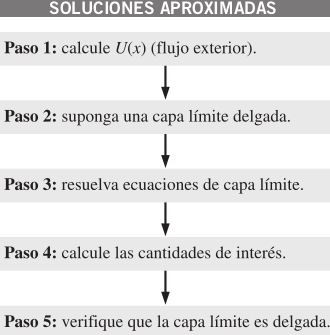
\includegraphics[scale=0.25]{Section_Files/S3-imagenes-Jhon/0202.png}
\caption{Resumen del procedimiento de capa límite, para capas límite bidimensionales de flujo estacionario e incompresible en el plano $xy$.}
\end{figure}
{\tiny Mecánica de fluidos por Yunus A. Cengel, John M. Cimbala, pág. 540}
\end{frame}

%***************************

\begin{frame}{Espesor de desplazamiento}
\justifying
\begin{figure}[H]
\centering
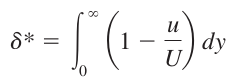
\includegraphics[scale=0.25]{Section_Files/S3-imagenes-Jhon/0211.png}
\caption{Espesor de desplazamiento}
\end{figure}
%\\
{\tiny Mecánica de fluidos por Yunus A. Cengel, John M. Cimbala, pág. 544}
\end{frame}

%***************************

\begin{frame}{Espesor de la cantidad de movimiento}
\justifying
\begin{figure}[H]
\centering
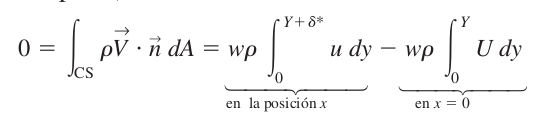
\includegraphics[scale=0.25]{Section_Files/S3-imagenes-Jhon/0219.png}
\caption{Espesor de desplazamiento}
\end{figure}
{\tiny Mecánica de fluidos por Yunus A. Cengel, John M. Cimbala, pág. 547}
\end{frame}

%***************************

\begin{frame}{Capa límite turbulenta sobre una placa plana}
\justifying
\begin{figure}[H]
\centering
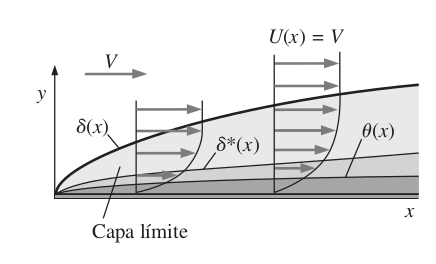
\includegraphics[scale=0.25]{Section_Files/S3-imagenes-Jhon/0231.png}
\caption{Para una capa límite laminar sobre placa plana, el espesor de desplazamiento es 35.0 por ciento de $ \delta $, y el espesor de la cantidad de movimiento es 13.5 por ciento de $ \delta $. }
\end{figure}
{\tiny Mecánica de fluidos por Yunus A. Cengel, John M. Cimbala, pág. 548}
\end{frame}

%***************************

\begin{frame}{Capas límite con gradientes de presión}
\justifying
\begin{figure}[H]
\centering
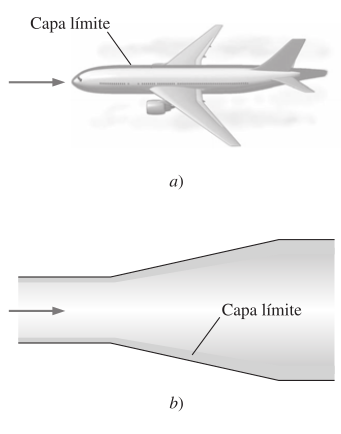
\includegraphics[scale=0.25]{Section_Files/S3-imagenes-Jhon/0245.png}
\caption{Las capas limite con gradientes de presión distintos de cero ocurren tanto en flujos externos como en internos: a) capa límite que se forma a lo largo del fuselaje de un avión y hacia la estela, y b) capa límite que crece a lo largo de la pared de un difusor (en abmos casos está exagerado el espesor de la capa límite).}
\end{figure}
{\tiny Mecánica de fluidos por Yunus A. Cengel, John M. Cimbala, pág. 554}
\end{frame}

%***************************

\begin{frame}{Técnica de la integral de la cantidad de movimiento para capas límite}
\begin{figure}[H]
\centering
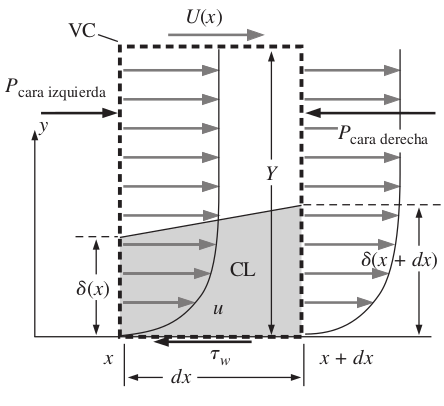
\includegraphics[scale=0.25]{Section_Files/S3-imagenes-Jhon/0259.png}
\caption{Volumen de control (línea negra punteada gruesa) que se usa en la deducción de la ecuación integral de la cantidad de movimiento (CL se refiere a capa límite.}
\end{figure}
{\tiny Mecánica de fluidos por Yunus A. Cengel, John M. Cimbala, pág. 559}
\end{frame}